%-----------------------------------------------------------------
\section{Packs}
\label{sec:packs}
%-----------------------------------------------------------------

%+-+-+-+-+-+-+-+-+-+-+-+-+-+-+-+-+-+-+-+-+-+-+-+-+-+-+-+-+-+-+-+-+
\subsection{[FLEX110] FLEX multibus pack}
\label{subsec:110}
%+-+-+-+-+-+-+-+-+-+-+-+-+-+-+-+-+-+-+-+-+-+-+-+-+-+-+-+-+-+-+-+-+
The FLEX multibus pack, depicted in the Figure ~\ref{fig:flex110}, with most widely used serial communication standards is now available!\\

\begin{figure}[!ht]
	\centering
		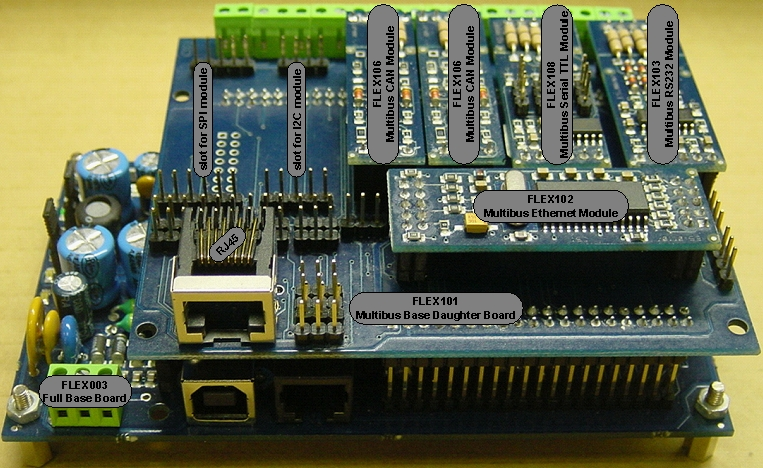
\includegraphics[width=0.90\textwidth, bb=0 0 763 468]{images/flex110.jpg}
	\caption{[FLEX110] FLEX multibus pack}
	\label{fig:flex110}
\end{figure}

\noindent The FLEX Multibus Base Daughter Board is piggybacked on FLEX Base Boards (FLEX Full, refer Subsection ~\ref{subsec:001}/FLEX Light refer Subsection ~\ref{subsec:003}) and in turn, the FLEX Multibus modules are piggybacked on the FLEX Multibus Base Daughter Board.\\

\noindent The FLEX multibus pack consists of:
\begin{itemize}
  \item 1 x [FLEX101] FLEX Multibus Base Daughter Board (bare board without Ethernet port), refer Subsection ~\ref{subsec:101}
  \item 1 x [FLEX102] FLEX Multibus Ethernet Module + 1 x RJ45 Ethernet port (to be soldered), refer Subsection ~\ref{subsec:102}
  \item 2 x [FLEX103] FLEX Multibus RS232 Modules, refer Subsection ~\ref{subsec:103}
  \item 1 x [FLEX104] FLEX Multibus RS485 Module, refer Subsection ~\ref{subsec:104}
  \item 1 x [FLEX105] FLEX Multibus RS422 Module, refer Subsection ~\ref{subsec:105}
  \item 2 x [FLEX106] FLEX Multibus CAN Modules, refer Subsection ~\ref{subsec:106}
  \item 1 x [FLEX107] FLEX Multibus SPI Module, refer Subsection ~\ref{subsec:107}
  \item 1 x [FLEX108] FLEX Multibus Serial TTL Module, refer Subsection ~\ref{subsec:108}
\end{itemize}

{\tt Note: The FLEX multibus pack does not include FLEX Base Board.}\\


%^^^^^^^^^^^^^^^^^^^^^^^^^^^^^^^^^^^^^^^^^^^^^^^^^^
\subsubsection{Technical details}
\label{subsubsec:110tech}
%^^^^^^^^^^^^^^^^^^^^^^^^^^^^^^^^^^^^^^^^^^^^^^^^^^
Refer technical details of:\\
\indent $\bullet$ \hspace{0.1cm} [FLEX101] FLEX Multibus Base Daughter Board, refer Sub-subsection ~\ref{subsubsec:101tech}\\
\indent $\bullet$ \hspace{0.1cm} [FLEX102] FLEX Multibus Ethernet Module, refer Sub-subsection ~\ref{subsubsec:102tech}\\
\indent $\bullet$ \hspace{0.1cm} [FLEX103] FLEX Multibus RS232 Module, refer Sub-subsection ~\ref{subsubsec:103tech}\\
\indent $\bullet$ \hspace{0.1cm} [FLEX104] FLEX Multibus RS485 Module, refer Sub-subsection ~\ref{subsubsec:104tech}\\
\indent $\bullet$ \hspace{0.1cm} [FLEX105] FLEX Multibus RS422 Module, refer Sub-subsection ~\ref{subsubsec:105tech}\\
\indent $\bullet$ \hspace{0.1cm} [FLEX106] FLEX Multibus CAN Modules, refer Sub-subsection ~\ref{subsubsec:106tech}\\
\indent $\bullet$ \hspace{0.1cm} [FLEX107] FLEX Multibus SPI Module, refer Sub-subsection ~\ref{subsubsec:107tech}\\
\indent $\bullet$ \hspace{0.1cm} [FLEX108] FLEX Multibus Serial TTL Module, refer Sub-subsection ~\ref{subsubsec:108tech}\\




%+-+-+-+-+-+-+-+-+-+-+-+-+-+-+-+-+-+-+-+-+-+-+-+-+-+-+-+-+-+-+-+-+
\clearpage
\subsection{[FLEX111] FLEX fast track suite}
\label{subsec:111}
%+-+-+-+-+-+-+-+-+-+-+-+-+-+-+-+-+-+-+-+-+-+-+-+-+-+-+-+-+-+-+-+-+
FLEX boards enable easy and fast development of embedded applications for the Microchip dsPIC� DSC micro-controller. The easily expandable hardware, combined with widely available software applications, makes FLEX ideal for Schools and Universities for fast track education.\\

\begin{figure}[!ht]
	\centering
		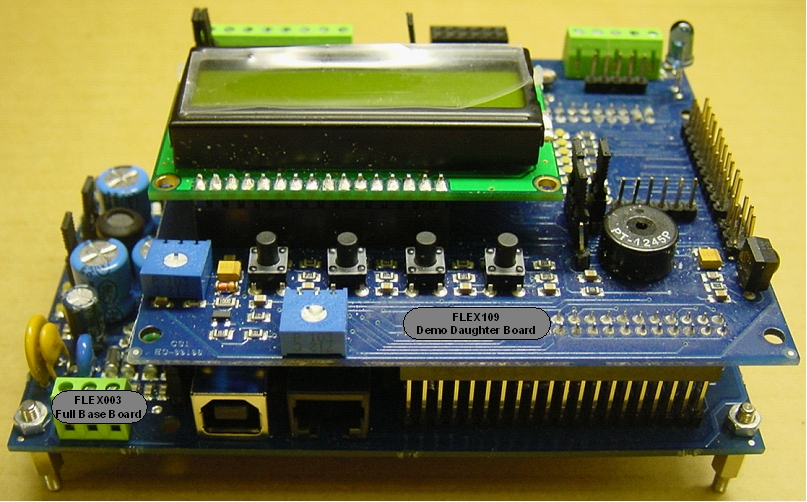
\includegraphics[width=0.90\textwidth, bb=0 0 807 502]{images/flex111.jpg}
	\caption{[FLEX111] FLEX fast track suite}
	\label{fig:flex111}
\end{figure}

\noindent As depicted in the Figure ~\ref{fig:flex111}, the FLEX Demo Daughter Board is one of the few educational boards offering 2 DAC outputs, a 3-axis accelerometer, and a direct support for an encoder. Moreover, with the direct support of the Scilab code generator, applications can be entirely generated without writing any C code.\\

\noindent The FLEX fast track suite consists of:
\begin{itemize}
  \item Hardware
    \begin{itemize}
      \item 1 x [FLEX003] FLEX Full Base Board, refer Subsection ~\ref{subsec:003}
      \item 1 x [FLEX109] FLEX Demo Daughter Board, refer Subsection ~\ref{subsec:109}
    \end{itemize}
  \item Free Software
    \begin{itemize}
      \item ERIKA Enterprise real-time kernel
      \item Scilab/Scicos simulation and code generation tool
    \end{itemize}
  \item Support (available on the web-site)
    \begin{itemize}
      \item Ready to run demos with source code
      \item Application notes
      \item User Forums
      \item Wiki
    \end{itemize}
\end{itemize}


%^^^^^^^^^^^^^^^^^^^^^^^^^^^^^^^^^^^^^^^^^^^^^^^^^^
\subsubsection{Technical details}
\label{subsubsec:111tech}
%^^^^^^^^^^^^^^^^^^^^^^^^^^^^^^^^^^^^^^^^^^^^^^^^^^
Refer technical details of:\\
\indent $\bullet$ \hspace{0.1cm} [FLEX003] FLEX Full Base Board, refer Sub-subsection ~\ref{subsubsec:003tech}\\
\indent $\bullet$ \hspace{0.1cm} [FLEX109] FLEX Demo Daughter Board, refer Sub-subsection ~\ref{subsubsec:109tech}\\